This section treats the repository as a set of distinct but coordinated state surfaces. The distinction matters because the system does not merely store one evolving manuscript; it maintains imported source material, generated section payloads, build outputs, runtime logs, media requests, and diagram memory as separate records with different ownership and update rules.

Imported source material is the raw input to the authoring process. It may arrive as markdown notes, outline fragments, or other human-authored text, and it should be preserved as source rather than silently rewritten into final prose. In the Codynamic Book Machine, imported material is useful precisely because it remains inspectable: it shows what was given to the system before normalization, drafting, or editorial repair.

Generated section payloads are different. A section payload is the \LaTeX{} body written for one section file, such as the content stored under \texttt{tex/section\_payloads/\{section\_id\}.tex}. This payload is not a transcript of the source notes; it is the section's authored output after the system has interpreted the outline, applied the section's intent, and converted the result into valid \LaTeX{}. Keeping payloads separate from source material makes revision tractable, because the system can compare what was imported with what was generated without conflating the two.

Build outputs form another surface. These are the compiled artifacts produced from the \LaTeX{} payloads, including intermediate files and the final document output. They answer a different question from the section payloads: not what the section says, but whether the manuscript assembles successfully and renders as intended. A clean payload can still produce a failed build, and a successful build can still conceal a weak section draft, so build outputs must remain independently visible.

Runtime logs are the operational memory of the system. They record task execution, message routing, callbacks, and failures as they happen. Unlike the manuscript itself, logs are not part of the book's argument; they are evidence of how the book was assembled. This makes them essential for debugging and for later editorial review, because they show which agent acted, what task was selected, and where a workflow stalled or branched.

Media requests occupy a separate surface because they are not yet artifacts. A request for a diagram, figure, or other media object is a structured handoff that describes what should be created, why it is needed, and how it should relate to the surrounding section. The request is not the diagram itself, and it should not be treated as if the visual already exists. That separation allows the system to track pending visual work without polluting the manuscript with invented paths or placeholder assets.

Diagram memory is the final surface in this section's account. Once a diagram is created, the diagram agent retains a durable record of its purpose, layout, node labels, edge relations, file path, and distinctness rationale. This memory prevents redundant visuals and helps later agents understand why a figure exists and how it differs from earlier diagrams. In other words, the diagram is not only an image file; it is also a remembered design decision.

These surfaces are coordinated rather than merged. Source material feeds section payloads; section payloads feed build outputs; logs record the transitions between them; media requests and diagram memory manage visual work across time. The architecture depends on this separation because each surface has a different lifecycle, a different owner, and a different failure mode. By keeping them distinct, the Codynamic Book Machine can revise prose, repair builds, route visuals, and audit execution without losing the provenance of any one layer of state.

Figure~\ref{fig:state-surfaces} summarizes the relationship among the main surfaces discussed here: imported source is normalized into section payloads, payloads are compiled into build artifacts, logs observe the transitions, and media requests plus diagram memory manage visual work across the same workflow.

\begin{figure}[htbp]
\centering
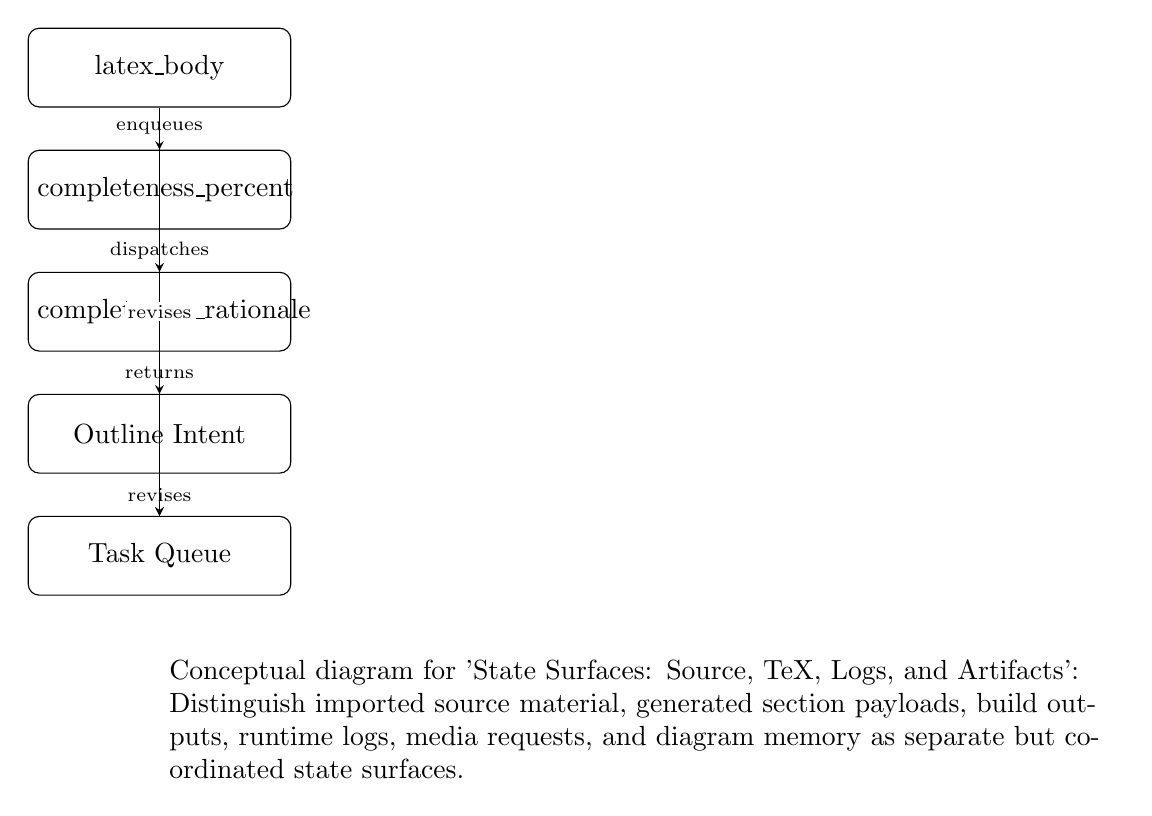
\begin{tikzpicture}[>=stealth, node distance=2.2cm,
  concept/.style={draw, rounded corners, align=center, text width=3.1cm, minimum height=1cm},
  relation/.style={font=\scriptsize, fill=white, inner sep=1pt}]
\node[concept] (n1) at (0,0.0) {latex\_body};
\node[concept] (n2) at (0,-1.55) {completeness\_percent};
\node[concept] (n3) at (0,-3.1) {completeness\_rationale};
\node[concept] (n4) at (0,-4.65) {Outline Intent};
\node[concept] (n5) at (0,-6.2) {Task Queue};
\draw[->] (n1) -- node[relation] {enqueues} (n2);
\draw[->] (n2) -- node[relation] {dispatches} (n3);
\draw[->] (n3) -- node[relation] {returns} (n4);
\draw[->] (n4) -- node[relation] {revises} (n5);
\draw[->] (n1) -- node[relation] {revises} (n5);
\node[align=left, text width=12cm, anchor=north west] at (0,-7.4) {Conceptual diagram for 'State Surfaces: Source, TeX, Logs, and Artifacts': Distinguish imported source material, generated section payloads, build outputs, runtime logs, media requests, and diagram memory as separate but coordinated state surfaces.};
\end{tikzpicture}

\caption{Conceptual diagram for ``State Surfaces: Source, TeX, Logs, and Artifacts'': Distinguish imported source material, generated section payloads, build outputs, runtime logs, media requests, and diagram memory as separate but coordinated state surfaces.}
\label{fig:state-surfaces}
\end{figure}
